\documentclass[../../main.tex]{subfiles}

\begin{document}
    %
    An vielen Stellen im alltäglichen Leben ziehst du irgendwelche Schlussfolgerungen -- die meisten davon, ohne wirklich darüber nachzudenken. Dauernd leitest du aus deinen Beobachtungen Informationen ab. Alleine schon die Erkenntnis, dass du Hunger hast, weil du hörst, dass dein Magen knurrt, ist eine Schlussfolgerung. Ähnlich ist es in der Mathematik unabdingbar, dass du ausgehend von Beobachtungen oder gegebenen Aussagen auf neue Aussagen schließen kannst. Du lernst in diesem Kapitel die \emph{Aussagenlogik} kennen, die systematisch an das Schlussfolgern herangeht und damit ein wichtiges Werkzeug für Schlussfolgerungen in der Mathematik ist.
    
    Der Hauptzweck der Aussagenlogik ist es, dir als Werkzeug für Schlussfolgerungen (nicht nur) in der Mathematik zur Verfügung zu stehen. Im Verlauf des Kapitels wird dir auffallen, dass die deutsche Sprache an viele Stellen zu uneindeutig und unübersichtlich ist, um komplexere Schlussfolgerungen übersichtlich nachvollziehbar zu machen. Was sind zum Beispiel deine Optionen, wenn die Speisekarte \enquote{Einen Burger und Pommes oder Salat} anbietet? Die zwei möglichen Interpretationen für die Speisekarte sind, dass du wählen darfst zwischen\dots
    \begin{itemize}[label=\dots, nosep]
        \item dem Burger mit Pommes oder dem Burger mit Salat.
        \item dem Burger mit Pommes oder nur dem Salat (ohne Burger).
    \end{itemize}
    Die zweite Option wird wohl nicht gemeint sein, aber ist dennoch eine mögliche Interpretation. Wir betrachten nun weitere Beispiele, in denen wir vorerst natürlichsprachlich Schlussfolgerungen ziehen. Im Verlauf dieses Kapitels findest du heraus, wie du dieselben und auch einige weniger offensichtliche Schlussfolgerungen ziehen kannst, indem du mithilfe mathematischer Formeln arbeitest, um deine Informationen eindeutig und übersichtlich zu halten.
    %
    
    %An vielen Stellen im alltäglichen Leben ziehst du irgendwelche Schlussfolgerungen -- die meisten davon, ohne wirklich darüber nachzudenken. Du kombinierst Informationen, die dir zur Verfügung stehen, und baust dadurch neue Informationen zusammen. Dieses Kapitel trägt den Namen \enquote{Aussagenlogik}. Die Aussagenlogik ist ein Werkzeug, das dir hilft, strukturiert zu schlussfolgern. Sehen wir uns zunächst ein erstes Beispiel an, das dir zeigt, wie solche Schlussfolgerungen aussehen können.
    
    % Im nächsten Absatz könnte man dann die ersten beiden Sätze streichen, weil sie jetzt hier sind. Dieser Vorschlag kommt, weil ich den jetzigen Einstieg etwas kurz finde -- da würde ein Satz mehr vermutlich nicht schaden. Ist zumindest mein persönlicher Geschmack und die Überlegung, wie ich das geschrieben hätte - Tobi
    
    %In diesem Kapitel lernst du, richtig zu schlussfolgern. Vielleicht ist es dir noch gar nicht bewusst, aber du kannst bereits einfache Schlussfolgerungen ziehen.
    
    \begin{example}{}
         \parpic[r]{
            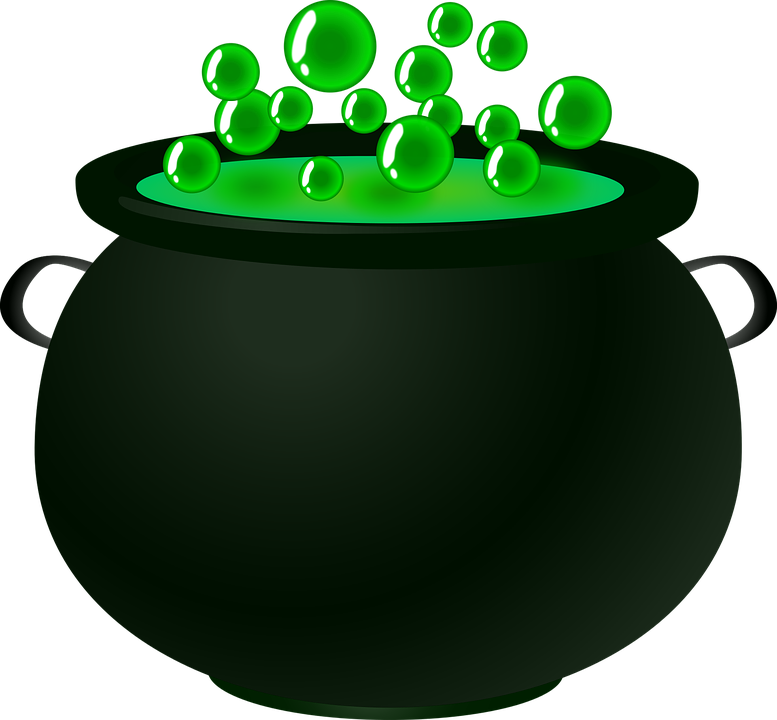
\includegraphics[width=0.2\textwidth]{images/zaubertrank.png}
        }
        Du hast einen Zaubertrank gefunden, von dem du weißt, dass er giftig für Menschen ist. Da du ein Mensch bist, schließt du daraus, dass der Zaubertrank für dich giftig sein wird.
        
        \picskip{3}
        Später finden ein Freund von dir und du zwei identisch aussehende Zaubertränke. Ihr wisst wieder aus sicherer Quelle, dass einer der Tränke Flügel verleiht und der andere giftig ist. Dein Freund hat einen der Zaubertränke getrunken und ihm sind Flügel gewachsen. Du folgerst also, dass der übrig gebliebene Zaubertrank giftig sein muss.
    \end{example}
    
    %Old version:
    %\begin{example}{}
    %     \parpic[r]{
    %        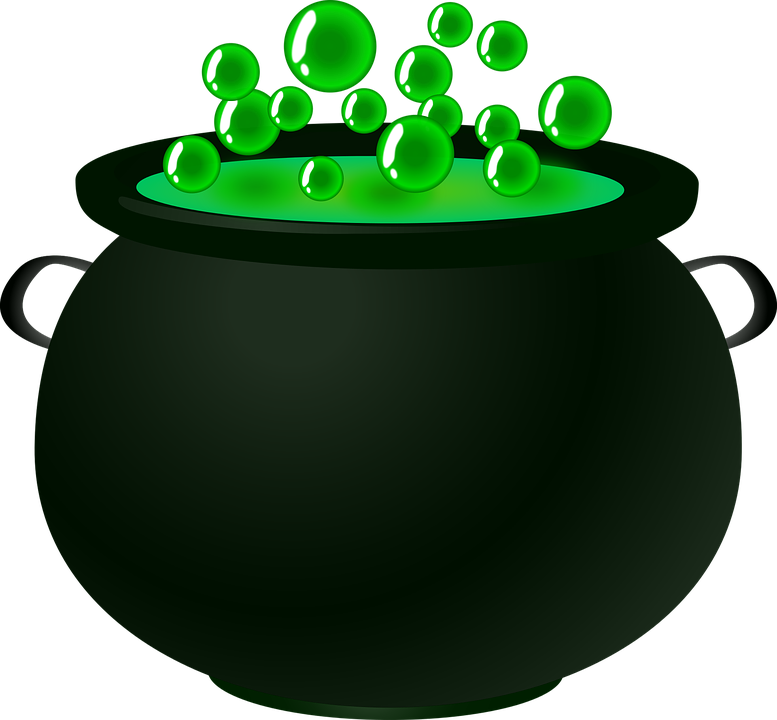
\includegraphics[width=0.2\textwidth]{images/Zaubertrank.png}
    %    }
    %    Stelle dir vor, du hast einen Zaubertrank gefunden und du weißt aus sicherer Quelle, dass dieser Zaubertrank giftig ist für Menschen. Da du ein Mensch bist, schließt du daraus, dass der Zaubertrank für dich giftig sein wird. Damit hast du bereits 
    %    logisch geschlussfolgert.
    %    \\ \\
    %    Stelle dir weiter vor, dass du und dein Freund zwei identisch aussehende Zaubertränke gefunden habt. Ihr wisst wieder aus sicherer Quelle, dass einer der Tränke Flügel verleiht und der andere giftig ist. Dein Freund hat einen der Zaubertränke getrunken und ihm sind Flügel gewachsen. Du folgerst also, dass der übrig gebliebene Zaubertrank giftig sein muss. Das ist wieder eine Schlussfolgerung.
    %\end{example}

    %Dieses Kapitel trägt den Namen \enquote{Aussagenlogik}. Die Aussagenlogik ist ein Werkzeug, das dir hilft strukturiert zu schlussfolgern. 
    Zugegebenermaßen waren die Schlussfolgerungen, die hier angestellt worden sind, ziemlich simpel. Doch logische Folgerungen zu ziehen, ist nicht immer so einfach. Das nächste Beispiel ist ein schwierigeres Logikrätsel. Mit den Methoden, die in diesem Kapitel vorgestellt werden, wirst du später in der Lage sein, solche Rätsel systematisch zu lösen.
    
    \begin{example}{}
        \parpic[r]{
            
\includegraphics[width=0.2\textwidth]{images/wizard.png}
        }
        
        Ein Zauberer gibt dir einen Zaubertrank, der entweder giftig ist oder dir Flügel verleiht. Der Zauberer sagt entweder immer die Wahrheit oder lügt immer.
        
        Er gestattet dir \emph{eine} Frage, um herauszufinden, ob der Zaubertrank giftig ist oder dir Flügel verleiht.
        
        \picskip{1}
        Natürlich möchtest du den Trank nur dann trinken, wenn er \emph{nicht} giftig ist. \textbf{Welche Frage musst du dem Zauberer also stellen, um herauszufinden, ob der Trank giftig ist?}
        
        Mithilfe von aussagenlogischen Überlegungen wirst du im Laufe des Kapitels in der Lage sein, systematisch herauszufinden, was du den Zauberer fragen musst.
    \end{example}
    
    Die Aussagenlogik beschäftigt sich mit Aussagen. Das sind Sätze, die zwar keine Fragen sind, auf die man aber trotzdem entweder mit \enquote{Ja, das ist \textbf{wahr}} oder \enquote{Nein, das ist \textbf{falsch}} antworten könnte. Ergeben beide diese Antwortmöglichkeiten auf einen Satz keinen Sinn, dann ist dieser Satz keine Aussage.
    \begin{example}{}
        Stell dir vor du hast wieder einen giftigen Zaubertrank gefunden. Dann ist der Satz
        \[\textrm{\enquote{Der Zaubertrank ist giftig}}\]
        eine Aussage.
        Im Gespräch könnte man nämlich auf diesen Satz sowohl mit \enquote{Ja, das ist \textbf{wahr}} als auch mit \enquote{Nein, das ist \textbf{falsch}} antworten. 
        Dadurch, dass wir aber wissen, dass der Zaubertrank tatsächlich giftig ist, kann man sagen, dass hier nur \enquote{Ja, das ist \textbf{wahr}} die passende bzw. stimmige Antwort der beiden ist. Es handelt sich hierbei also um eine \textbf{wahre} Aussage.
        
        Der Satz
        \[\textrm{\enquote{Der Zaubertrank ist harmlos}}\]
        ist ebenfalls eine Aussage. Der Zaubertrank ist giftig, also keineswegs harmlos. Man kann deshalb auf diesen Satz passend mit \enquote{Nein, das ist \textbf{falsch}} antworten. Es handelt sich demnach um eine \textbf{falsche} Aussage.
    \end{example}
    
    Aussagen sind also genau die Sätze, abgesehen von Fragen, auf die man entweder mit \enquote{Ja, das ist \textbf{wahr}} oder mit \enquote{Nein, das ist \textbf{falsch}} antworten kann. Kann man auf eine Aussage passend bzw. stimmig mit \enquote{Ja, das ist \textbf{wahr}} antworten, dann ist die Aussage \textbf{wahr}. Ist nur \enquote{Nein, das ist \textbf{falsch}} eine passende Antwort, dann ist die Aussage \textbf{falsch}.

    \begin{example}{}
        Wir schauen uns einmal Beispiele für Sätze an, die keine Aussagen sind. Das sind zum einen Aufforderungen wie
        \[\textrm{\enquote{Trinke diesen Zaubertrank!}}\]
        Dieser Aufforderung mit \enquote{Ja, das ist \textbf{wahr}} oder \enquote{Nein, das ist \textbf{falsch}} zu entgegnen, ergibt keinen Sinn. Unser natürliches Sprachgefühl sagt bereits, dass diese Antworten keine sinnvollen Fortsetzung des Gespräch sein können.
        
        Zwar kann man auf manche Fragen wie
         \[\textrm{\enquote{Ist der Zaubertrank giftig?}}\]
        mit \enquote{Ja, das ist \textbf{wahr}} oder \enquote{Nein, das ist \textbf{falsch}} antworten, jedoch wollen wir solche Sätze nicht als Aussagen bezeichnen. Solch eine Frage können wir nämlich auch einfach direkt als Aussage formulieren wie
        \enquote{Der Zaubertrank ist giftig}.
    \end{example}

    Es gibt Sätze auf die du entweder mit \enquote{Ja, das ist \textbf{wahr}} oder \enquote{Nein, das ist \textbf{falsch}} antworten könntest, jedoch nicht weißt welche die passende bzw. stimmige Antwort ist. Nichtsdestotrotz handelt es sich bei dem Satz um eine Aussage. Das, was einen Satz zur Aussage macht, ist, dass dieser mit \enquote{Ja, das ist \textbf{wahr}} oder mit \enquote{Nein, das ist \textbf{falsch}} bejaht bzw. verneint werden kann. Welche nun die passende Antwort ist, ist dabei belanglos.
   
   \begin{example}{}
        Der Satz 
        \[\textrm{\enquote{Der Zauberer ist 1024 Jahre alt}}\]
        ist eine Aussage. Zwar wissen wir eventuell nicht, ob der Zauberer tatsächlich 1024 Jahre alt ist (Der Zauberer verrät uns sein Alter nicht), nichtsdestotrotz ist dieser Satz eine Aussage. Das liegt daran, dass \enquote{Ja, das ist \textbf{wahr}} und  \enquote{Nein, das ist \textbf{falsch}} Antwortmöglichkeiten sind. Welche dieser beiden Antworten jetzt die passende ist, kann uns dabei egal sein.
   \end{example}

    Im Verlaufe dieses Kapitels werden wir Aussagen genauer untersuchen. Im nächsten Abschnitt nehmen wir die Struktur von Aussagen unter die Lupe und schauen wie diese aufgebaut sind. Im darauf folgenden Abschnitt beschäftigten wir uns damit wie man bei Aussagen entscheiden kann, ob diese wahr oder falsch sind. Am Ende kommen wir auf das Logikrätsel mit dem Zauberer zurück und nutzen das neu gewonnene Wissen, um dieses Rätsel systematisch mit der Aussagenlogik zu lösen.

    
    % Ist nur zum Ausprobieren hier
    %\begin{example}{}
     %   \[\underbrace{\text{Ich erhalte einen %Burger}}_{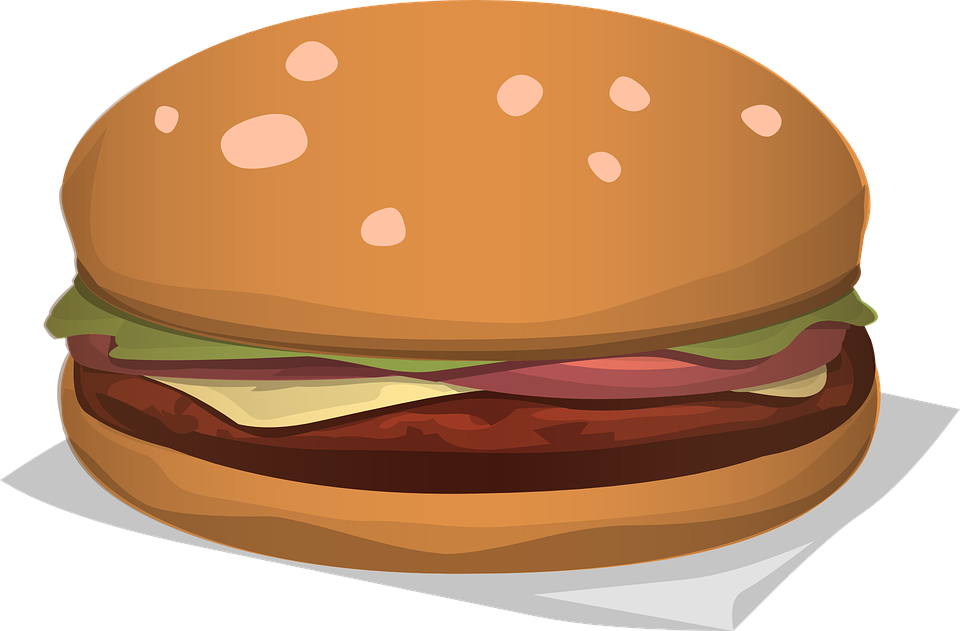
\includegraphics[height=1cm]{images/burger.png}}\text{~und~}\underbrace{\text{ich %erhalte Pommes}}_{
\includegraphics[height=1cm]{images/pommes.png}}\text{~oder~}\underbrace{\%text{ich erhalte einen Salat.}}_{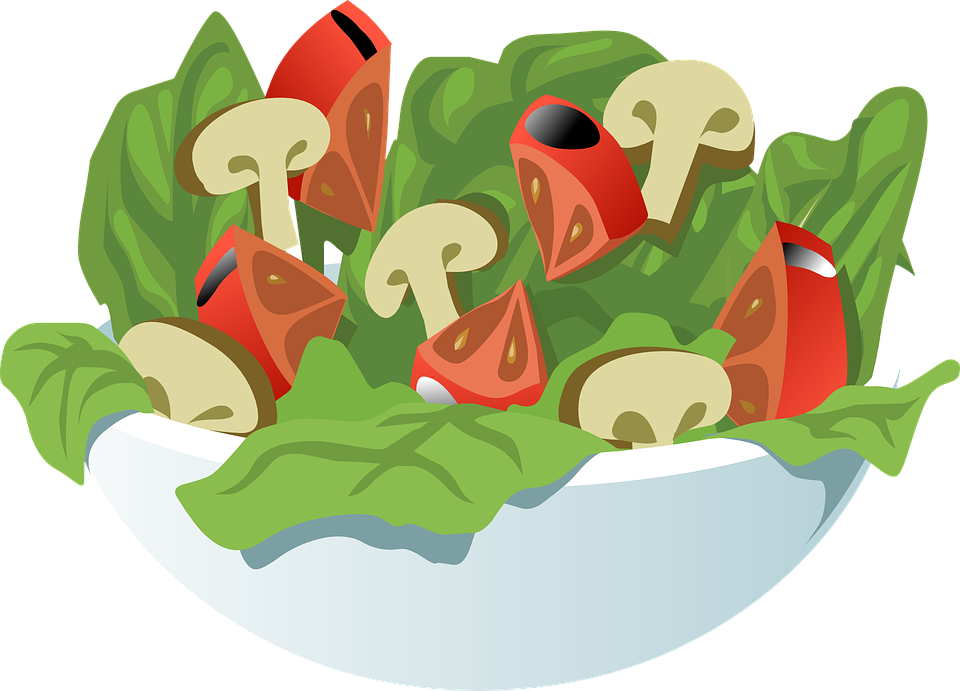
\includegraphics[height=1cm]{images/salat.png}}\]
    %\end{example}
        
\end{document}